Как мы уже говорили - обратные функции - это исходные повернутые на 90 градусов. В силу периодичности тригонометрических функций (также как было с параболой) - нарушается определение функции. По этому принято брать часть этих функций.  Например, у функции 
$y = \arcsin{x}$ область значений рассматривается лишь в промежутке $x \in [-\frac{\pi}{2},\frac{\pi}{2}]$

\begin{itemize}
    \item Арксинус $y = \arcsin{x}$. 
    \begin{figure}[h!]
    \centering
    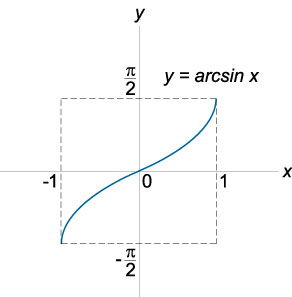
\includegraphics[width=0.5\textwidth]{img/arcsin.jpg}
    \end{figure}
    \item Арккосинус $y = \arccos{x}$
    \begin{figure}[h!]
    \centering
    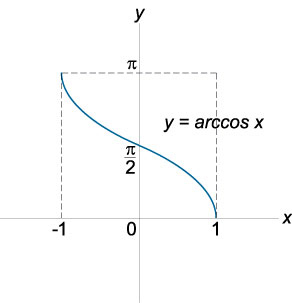
\includegraphics[width=0.5\textwidth]{img/arccos.jpg}
    \end{figure}
    \newpage
    \item Арктангенс $y = \arctg{x}$
    \begin{figure}[h!]
    \centering
    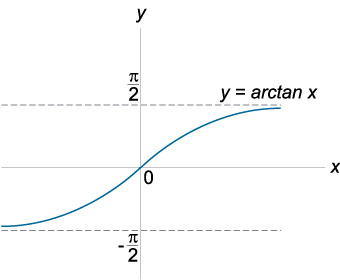
\includegraphics[width=0.5\textwidth]{img/arctg.jpg}
    \end{figure}
    \item Арккотангенс $y = \arcctg{x}$
    \begin{figure}[h!]
    \centering
    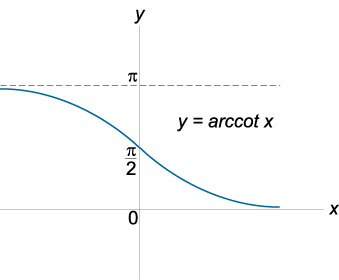
\includegraphics[width=0.5\textwidth]{img/arcctg.jpg}
    \end{figure}
\end{itemize}

(?) Какие D(y) и E(y) у представленных выше функций?